\documentclass[reqno]{amsart}
\usepackage{amscd, amssymb, amsmath, amsthm}
\usepackage{graphicx}
\usepackage[colorlinks=true,linkcolor=blue]{hyperref}
\usepackage[utf8]{inputenc}
\usepackage[T1]{fontenc}
\usepackage{textcomp}
\usepackage{babel}
%% for identity function 1:
\usepackage{bbm}
%%For category theory diagrams:
\usepackage{tikz-cd}
\usepackage{enumitem}


\setlength\parindent{0pt}

\pdfsuppresswarningpagegroup=1

\newtheorem{theorem}{Theorem}[section]
\newtheorem{lemma}[theorem]{Lemma}
\newtheorem{proposition}[theorem]{Proposition}
\newtheorem{corollary}[theorem]{Corollary}
\newtheorem{conjecture}[theorem]{Conjecture}

\theoremstyle{definition}
\newtheorem{definition}[theorem]{Definition}
\newtheorem{example}[theorem]{Example}
\newtheorem{exercise}[theorem]{Exercise}
\newtheorem{problem}[theorem]{Problem}
\newtheorem{question}[theorem]{Question}

\theoremstyle{remark}
\newtheorem*{remark}{Remark}
\newtheorem*{note}{Note}
\newtheorem*{solution}{Solution}



%Inequalities
\newcommand{\cycsum}{\sum_{\mathrm{cyc}}}
\newcommand{\symsum}{\sum_{\mathrm{sym}}}
\newcommand{\cycprod}{\prod_{\mathrm{cyc}}}
\newcommand{\symprod}{\prod_{\mathrm{sym}}}

%Linear Algebra

\DeclareMathOperator{\Span}{span}
\DeclareMathOperator{\Ima}{Im}
\DeclareMathOperator{\diag}{diag}
\DeclareMathOperator{\Ker}{Ker}
\DeclareMathOperator{\ob}{ob}
\DeclareMathOperator{\Hom}{Hom}
\DeclareMathOperator{\sk}{sk}
\DeclareMathOperator{\Vect}{Vect}
\DeclareMathOperator{\Set}{Set}
\DeclareMathOperator{\Group}{Group}
\DeclareMathOperator{\Ring}{Ring}
\DeclareMathOperator{\Ab}{Ab}
\DeclareMathOperator{\Top}{Top}
\DeclareMathOperator{\hTop}{hTop}
\DeclareMathOperator{\Htpy}{Htpy}
\DeclareMathOperator{\Cat}{Cat}
\DeclareMathOperator{\CAT}{CAT}
\DeclareMathOperator{\Cone}{Cone}
\DeclareMathOperator{\dom}{dom}
\DeclareMathOperator{\cod}{cod}
\DeclareMathOperator{\Aut}{Aut}
\DeclareMathOperator{\Mat}{Mat}
\DeclareMathOperator{\Fin}{Fin}
\DeclareMathOperator{\rel}{rel}
\DeclareMathOperator{\Int}{Int}
\DeclareMathOperator{\sgn}{sgn}

%Row operations
\newcommand{\elem}[1]{% elementary operations
\xrightarrow{\substack{#1}}%
}

\newcommand{\lelem}[1]{% elementary operations (left alignment)
\xrightarrow{\begin{subarray}{l}#1\end{subarray}}%
}

%SS
\DeclareMathOperator{\supp}{supp}
\DeclareMathOperator{\Var}{Var}

%NT
\DeclareMathOperator{\ord}{ord}

%Alg
\DeclareMathOperator{\Rad}{Rad}
\DeclareMathOperator{\Jac}{Jac}

%Misc
\newcommand{\SL}{{\mathrm{SL}}}
\newcommand{\mobgp}{{\mathrm{PSL}_2(\mathbb{C})}}
\newcommand{\id}{{\mathrm{id}}}
\newcommand{\Mod}{{\mathrm{Mod}}}
\newcommand{\ud}{{\mathrm{d}}}
\newcommand{\Vol}{{\mathrm{Vol}}}
\newcommand{\Area}{{\mathrm{Area}}}
\newcommand{\diam}{{\mathrm{diam}}}


\newcommand{\reg}{{\mathtt{reg}}}
\newcommand{\geo}{{\mathtt{geo}}}

\newcommand{\tori}{{\mathcal{T}}}
\newcommand{\cpn}{{\mathtt{c}}}
\newcommand{\pat}{{\mathtt{p}}}




\begin{document}
\section{Curves, Surfaces and Hyperbolic Geometry}
\subsection{Simple closed curves}
There is a bijective correspondence
\[
\left\{ 
    \begin{tabular}{c}
    Nontrivial\\
    conjugacy classes\\
    in $\pi_1 (S)$
\end{tabular}
\right\} 
\longleftrightarrow
\left\{ 
    \begin{tabular}{c}
        Nontrivial free\\
        homotopy classes of oriented\\
        closed curves in $S$
\end{tabular}
\right\} 
\] 

\begin{definition}[Primitive and multiple elements]
    An element $g$ of a group $G$ is \textit{primitive} if there
    does not exist any $h \in G$ so that $g = h^{k}$ for
    $\left| k \right| >1$. The property of being a primitive
    is a conjugacy class invariant. In particular, it makes
    sense to say that a closed curve in a surface is primitive.\\
    A closed curve in $S$ is a multiple if it is a map
    $S^{1} \to S$ that factors through the map
    $S^{1} \stackrel{\times n}{\to } S^{1}$ for
    $n >1$, i.e., there exists a map $\tilde{\alpha} \colon
    S^{1} \to S$ such that the following diagram commutes:
    \begin{equation*}
    \begin{tikzcd}
        S^{1} \ar[r, "\times n"] \ar[rr, bend left = 45, dashed,
        "\tilde{\alpha}"] & S^{1} \ar[r,
        "\alpha"] & S
    \end{tikzcd}
    \end{equation*}
\end{definition}

\begin{definition}[Lifts]
    We make a distinction between lifts: let $p \colon
    \tilde{S} \to S$ be a covering space. By a \textit{lift} of a closed
    curve $\alpha$ to $\tilde{S}$ we will always mean the image of
    a lift $\mathbb{R} \to \tilde{S}$ of the map
    $\alpha \circ \pi$ where $\pi \colon \mathbb{R} \to S^{1}$ is
    the usual covering map. I.e., a lift of $\alpha \colon
    S^{1} \to S$ is a map  $\tilde{\alpha} \colon \mathbb{R} \to 
    \tilde{S}$ such that the following diagram commutes
    \begin{equation*}
    \begin{tikzcd}
        & & \tilde{S} \ar[d, "p"]\\
        \mathbb{R} \ar[r, "\pi"'] \ar[rru, "\tilde{\alpha}"] & S^{1} \ar[r, 
        "\alpha"'] & S
    \end{tikzcd}
    \end{equation*}
    A lift is different from a \textit{path lift} which is
    a proper subset of a lift. Namely, it would be
    the restriction of $\tilde{\alpha}$ to some interval of
    $\mathbb{R}$ of length $2 \pi$ if the covering map
    $\pi$ is of the form $t \mapsto e^{it}$.
\end{definition}

Now suppose $p \colon \tilde{S} \to S$ is the universal cover
and $\alpha$ is a simple closed curve in $S$ that is
not a multiple of another closed curve. In this case, there
is a bijective correspondence
between cosets in $ \pi_1 (S)$
 of the infinite cyclic subgroup $\left<\alpha \right>$ and
 the lifts of $\alpha$. This can be seen as follows: first choose
 a basepoint $\alpha(1) =  x_0 \in S$
and
 some $\tilde{x_0} \in p^{-1}(x_0)$. There exists a unique lift
 $\tilde{\alpha}$ of $\alpha$ such that
 \begin{equation*}
 \begin{tikzcd}
     & & \tilde{S}\ar[d, "p"] \\
     \mathbb{R} \ar[r] \ar[rru, "\tilde{\alpha}"] & S^{1} \ar[r, "\alpha"] & S
 \end{tikzcd}
 \end{equation*}
 commutes and such that
 $\tilde{\alpha}(0) = \tilde{x} \in p^{-1}(\alpha \circ \pi (0))$
 for some specific $\tilde{x}$  \cite[Cor. 4.2]{Bredon}.
 But the set
 $p^{-1} \left( \alpha \circ \pi (0) \right) $ is in bijective
 correspondence with the loops in $\pi_1 (S)$ by the path lifting lemma. 
 Now, under which path lifts are the lifts the same? The lifts of
 $\alpha$ to two points $\tilde{x}, \tilde{y} \in 
 p^{-1}\left( \alpha \circ \pi (0) \right) $ will be the same if
 $\alpha^{k} \cdot \tilde{x} = \tilde{y}$ where
 $\cdot $ denotes the monodromy action of $\pi_1 (S)$ on
 the fiber. Now, there exist $\gamma_x$ and
 $\gamma_y$ in $\pi_1 (S)$ such that
 $\gamma_x \cdot \tilde{x_0} = \tilde{x}$ and
 $\gamma_y \cdot \tilde{x_0} = \tilde{y}$, so
 $\alpha^k \gamma_x = \gamma_y$. Hence the lifts
 corresponding to $\gamma_x$ and $\gamma_y$ are the same if and only
 if $\alpha^k \gamma_x = \gamma_y$ for some $k$, i.e. if and only if
 $\gamma_x = \gamma_y$ in $\pi_1(S) / \left<\alpha \right>$.\\
 \linebreak
 As usual, the group $\pi_1 (S)$ acts on the set of lifts
 of $\alpha$ by deck transformations, and this action agrees
 with the usual left action of $\pi_1 (S)$ on the
 cosets of $\left<\alpha \right>$. The stabilizer of the lift
 corresponding to the coset $\gamma \left<\alpha \right>$ is
 the cyclic group $\left<\gamma \alpha \gamma^{-1} \right>$. See
 figure~\ref{fig:lifts-of-paths}.

 \begin{figure}[http]
     \centering
     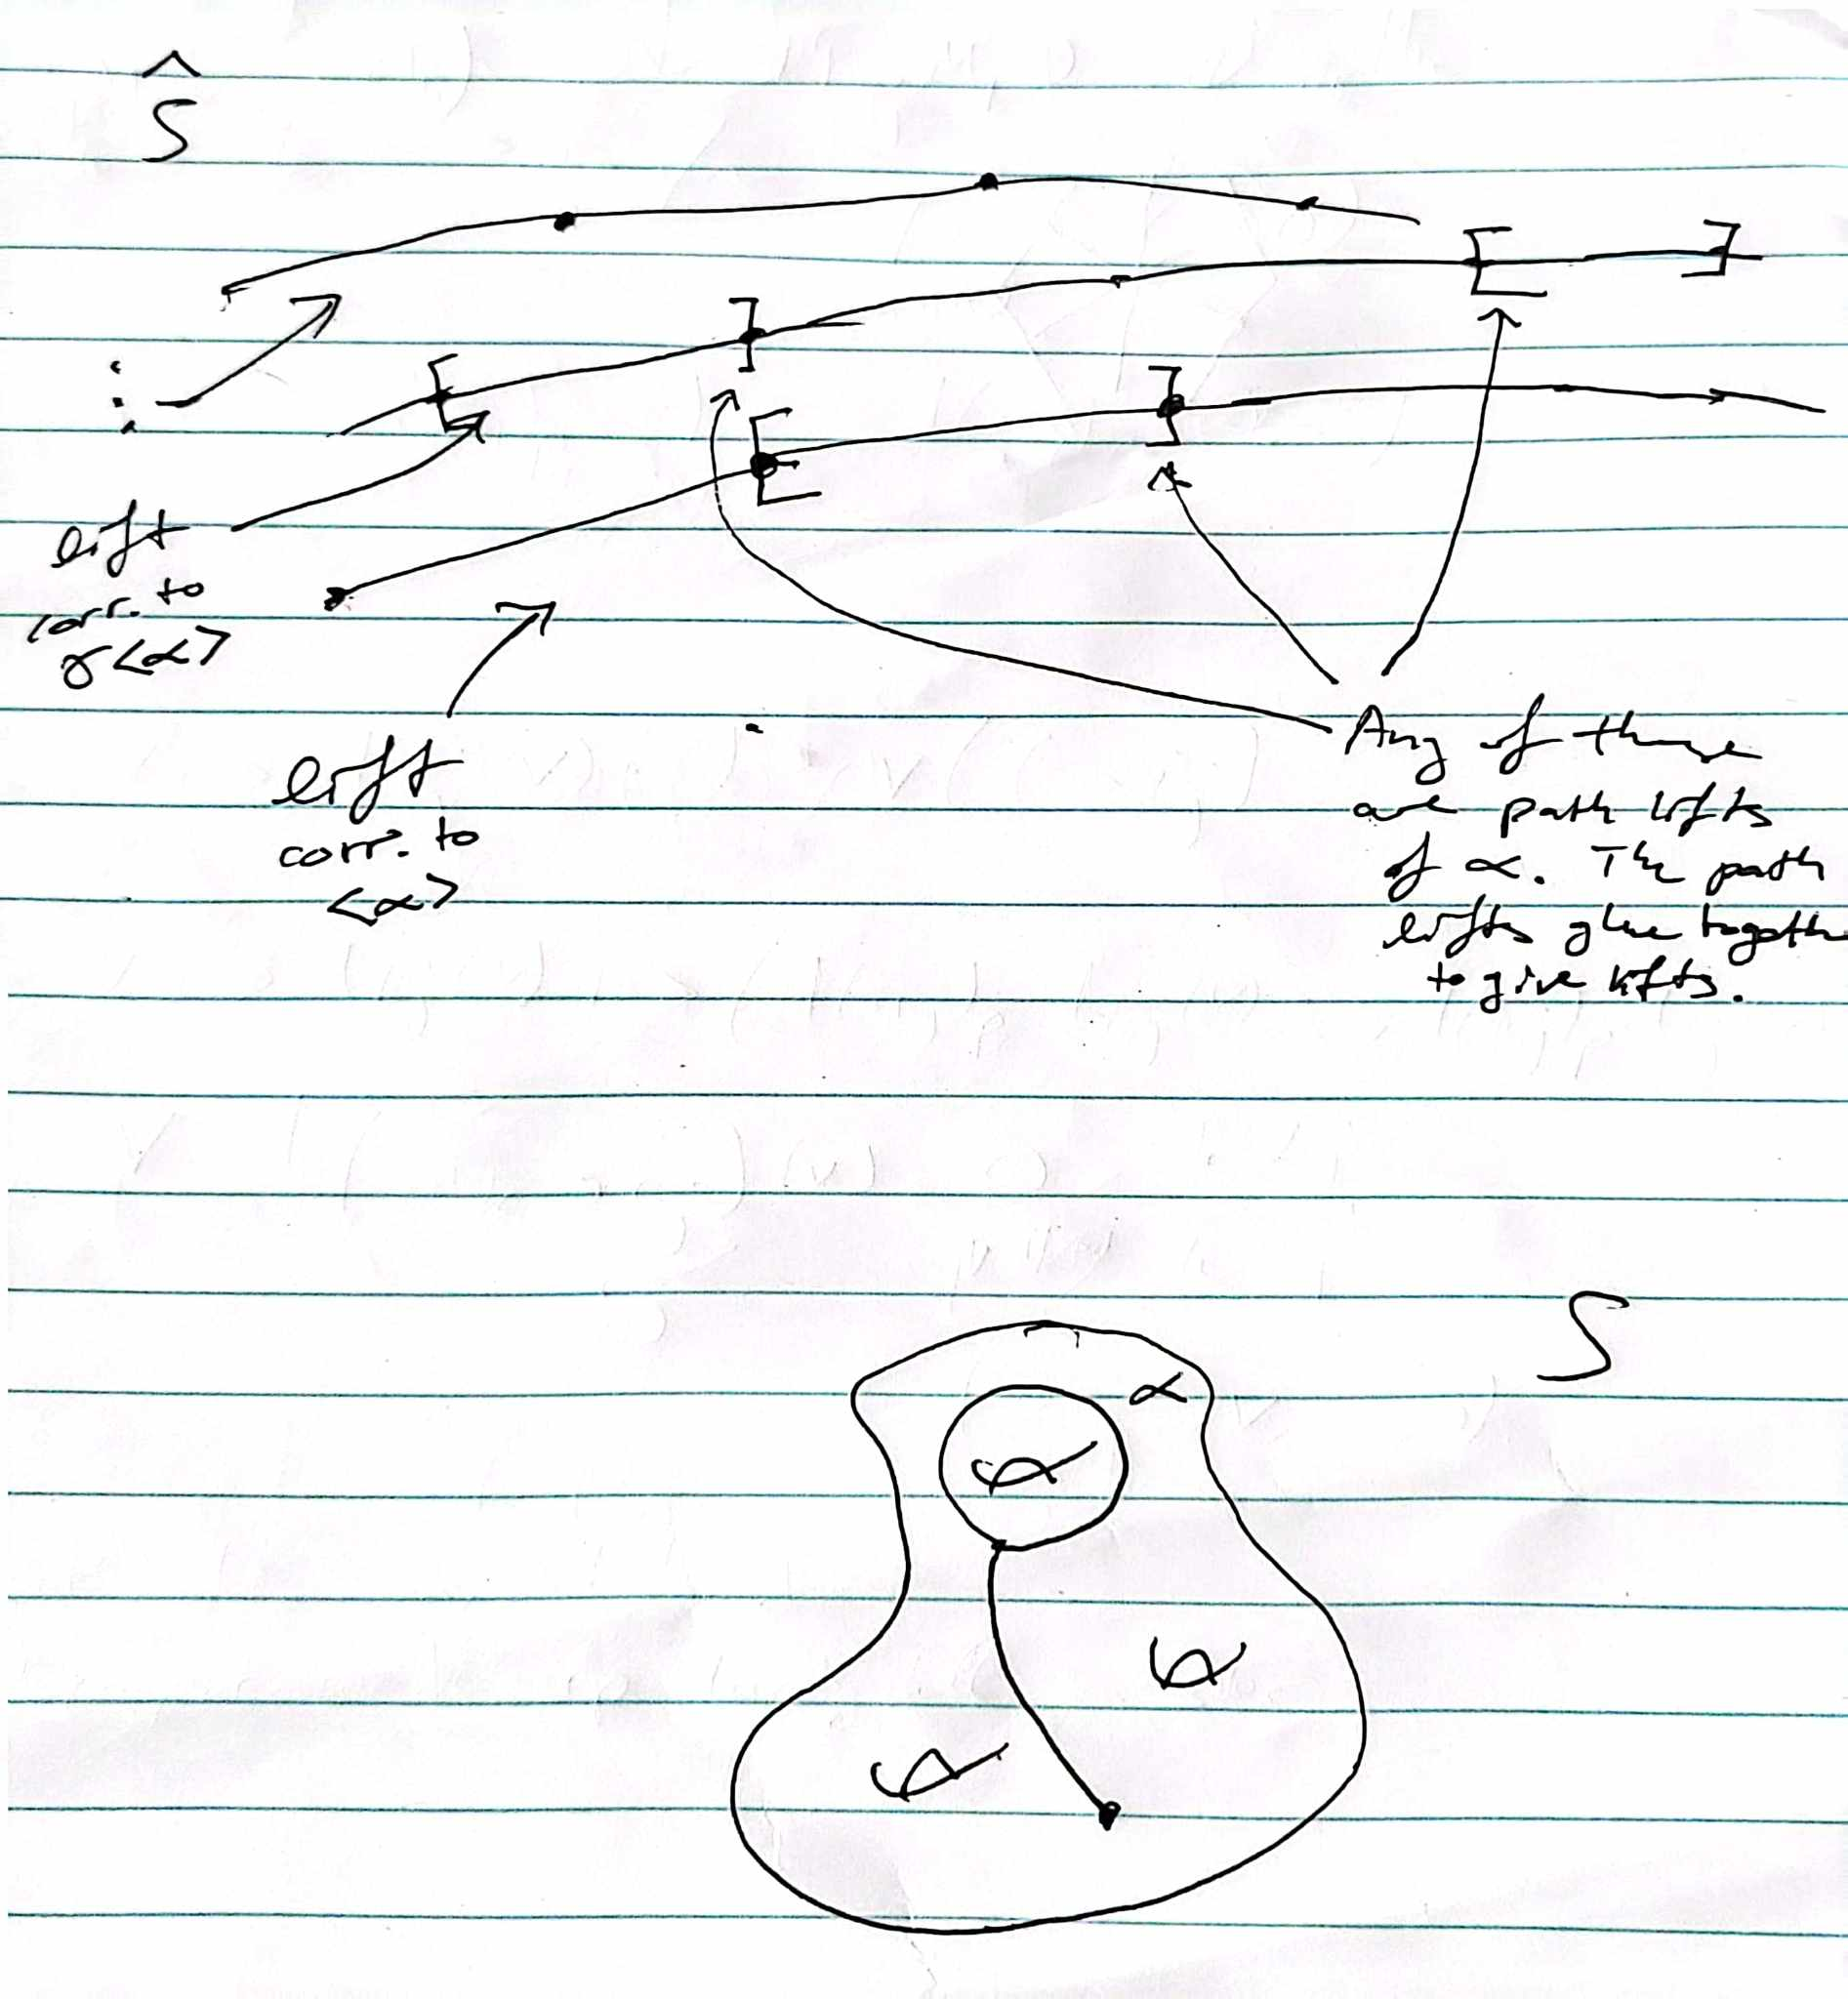
\includegraphics[width=0.8\textwidth]{lifts-of-paths.jpg}
     \caption{}
     \label{fig:lifts-of-paths}
 \end{figure}

Now we claim that when $S$ admits a hyperbolic metric and
$\alpha$ is a primitive element of $\pi_1 (S)$, we have
a bijective correspondence
\[
\left\{ 
    \begin{tabular}{c}
    Elements of the conjugacy\\
    class of $\alpha$ in $\pi_1 (S)$
\end{tabular}
\right\} 
\longleftrightarrow
\left\{ 
    \begin{tabular}{c}
    Lifts to $\tilde{S}$ of the\\
    closed curve $\alpha$
\end{tabular}
\right\} 
\] 
More precisely, we claim that the map which sends the lift
given by the coset $\gamma \left<\alpha \right>$ to
$\gamma \alpha \gamma^{-1}$ is bijective and well-defined.\\
To show that it is well-defined, suppose $\gamma \left<\alpha \right>$ and
$\beta \left<\alpha \right>$ give the same lift. Then
$\gamma = \beta \alpha^k$. So in particular,
\[
    \gamma \alpha \gamma^{-1} = \beta \alpha^k \alpha \alpha^{-k} \beta^{-1}
    = \beta \alpha \beta^{-1}
\] 
so they do correspond to the same element of the conjugacy class
$\left[ \alpha \right] $. It is clear that this is a surjective map.
Now suppose that $\gamma \alpha \gamma^{-1} = \beta \alpha \beta^{-1}$. 
Then $\beta^{-1} \gamma \alpha \left( \beta^{-1} \gamma \right)^{-1} =
\alpha$, so in particular, $\beta^{-1} \gamma \in C_{\pi_1(S)}(\alpha)$





 





\bibliography{mcg}
\end{document}
